\section{Performance Characteristics \punkte{30}}
% Port Usage
% We use the following notation for the port usage: 3*p015+1*p23, for example, denotes an instruction with four μops; three of these μops can each be executed on ports 0, 1, and 5, and one μop can be executed on ports 2 and 3.
% 1*p01
\subsection{Peak Performance}
As stated on the Compute Resources Webpage of the Institute of Computing \cite{noauthor_compute_nodate}, Rosa is a high performance computing cluster made up of 42 Nodes, each with two Intel XEON E5-2650 v3 CPUs with 10 cores each.
To calculate the Peak performance of the cluster, we begin by calculating the peak performance of a single core $P_{\text{core}}$ given by the equation \ref{eq:p_core}.
\begin{equation} \label{eq:p_core}
	\begin{aligned}
		P_{\text {core}} & =n_{\text {super}} \times n_{\text {FMA}} \times n_{\text {SIMD}} \times f \\
		                 & = 2 \times 2 \times 4 \times 2.3 \ \text{GHz}                              \\
		                 & = 36.8 \ \text{GFlops/s}
	\end{aligned}
\end{equation}
By consulting Intel's ARK website \cite{noauthor_intel_nodate} about the XEON E5-2650 v3 CPUs, we can find out further details about the CPU, firstly that it operates on a base frequency $f$ of $2.3$ GHz, secondly that it is part of the \textit{Haswell} microprocessor architecture family and thirdly that the CPU supports Intel's AVX2 SIMD instruction set extension.
The AVX2 SIMD instructions \cite{noauthor_intel_nodate-1} uses a 256-bit wide vector registers and because we consider 64-bit double precision float operations to compute the peak performance, each core is able to perform 4 operations simultaneously. Hence leading $n_{\text{SIMD}}$ to be 4.
Furthermore, by looking at the website uops.info \cite{noauthor_uopsinfo_nodate} and filtering the table using the keywords \texttt{Haswell} and \texttt{FMA} we can see that the throughput (TP) is 0.5, this means that a core can execute two float point operations per cycle, resulting in $n_{\text{super}} = 2$. In addition the port column shows \text{1*p01}, indicating that one vector FMA operation can be executed on each port 0 and 1. Hence we can set $n_{\text{FMA}}$ to 2 as well.\newline
\newline
After successfully calculating the peak performance of a single core, the result can now be used to compute the peak performance of a CPU, given by equation \ref{eq:pp-cpu}.
\begin{equation}\label{eq:pp-cpu}
	\begin{aligned}
		P_{\text{CPU}} & = n_{cores} \times P_{core}        \\
		               & = 10 \times 36.8 \ \text{GFlops/s} \\
		               & = 368 \ \text{GFlops/s}
	\end{aligned}
\end{equation}
The number of physical cores $n_{cores}$ can be found on the previously mentioned Intel ARK website \cite{noauthor_intel_nodate}.
Now we can compute the peak performance of a single Node on the Rosa cluster given by
\begin{equation}
	\begin{aligned}
		P_{\text{node}} & = n_{\text{sockets}} \times P_{\text{CPU}} \\
		                & =	2 \times  368 \ \text{GFlops/s}          \\
		                & =  736 \ \text{GFlops/s}.
	\end{aligned}
\end{equation}
$n_{\text{sockets}}$ can be set to 2, because for each we Node we have two sockets as stated on the USI's Institute for Computing website \cite{noauthor_compute_nodate}.
Now we are finally ready to compute the peak performance of the 42 node cluster giving us the final peak performance of
\begin{equation}
	\begin{aligned}
		P_{\text{Rosa}} & = n_{\text{nodes}} \times P_{\text{node}}              \\
		                & = 42 \times  736 \ \text{GFlops/s}                     \\
		                & =  30912 \ \text{GFlops/s} = 30.912 \ \text{TFlops/s}.
	\end{aligned}
\end{equation}

\subsection{Memory Hierarchies}
The memory hierarchy of a single node on the Rosa cluster can be seen in Figure \ref{fig:node}. It shows two identical CPU's with 10 cores and the corresponding Level of caches including their size.
\begin{figure}[H]
	\centering
	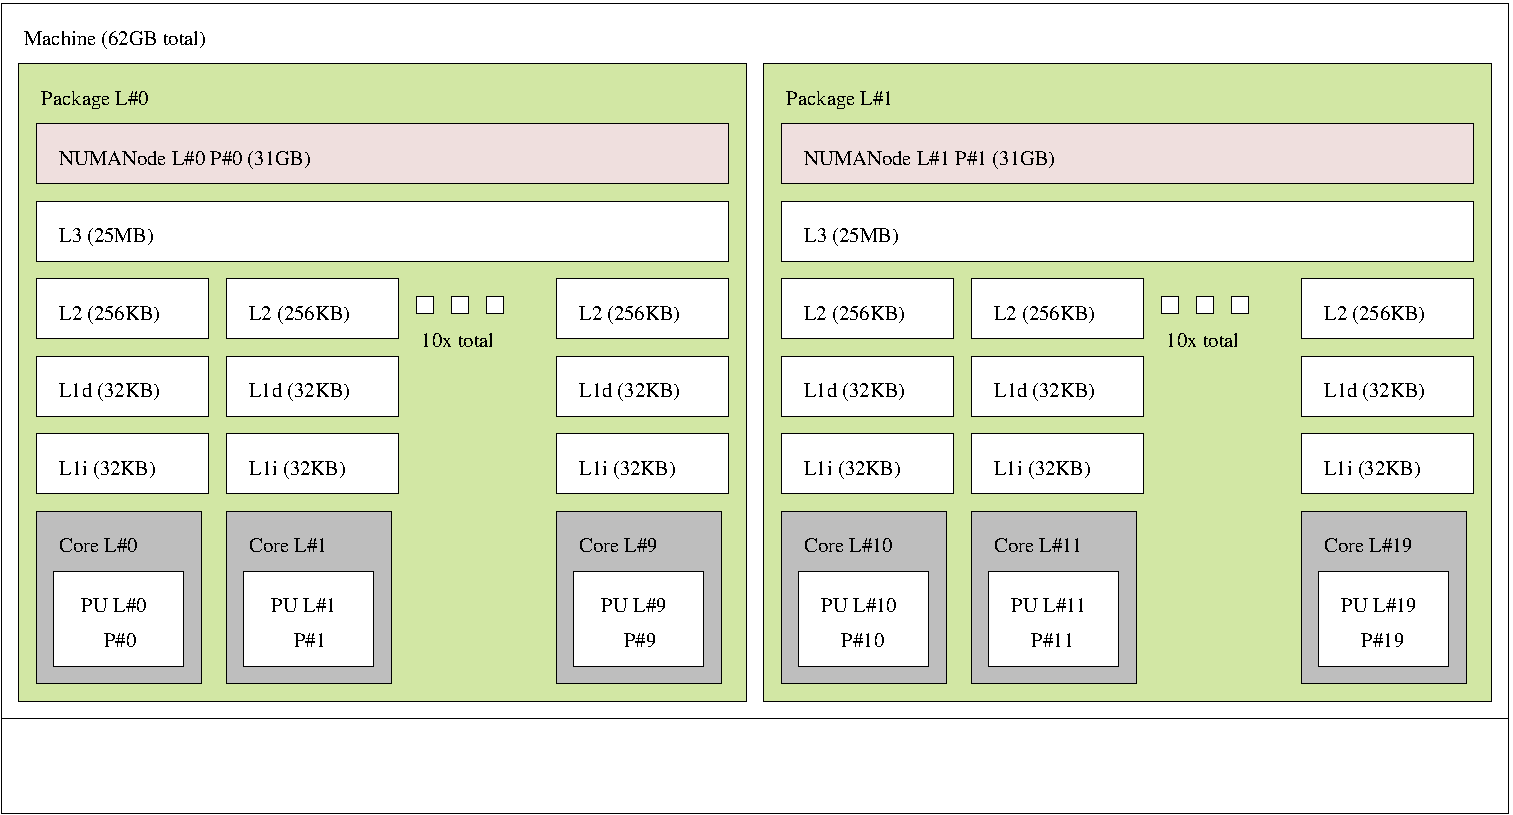
\includegraphics[width=\textwidth]{../media/XEON_E5-2650.pdf}
	\caption{2 x Intel Xeon E5-2650 v3 @ 2.30GHz, 20 (2 x 10) cores}
	\label{fig:node}
\end{figure}
For single core the memory hierarchy is summarized in Table \ref{tab:cache}.
\begin{table}[H]
	\centering
	\begin{tabular}{|l|r|}
		\hline
		Main Memory & 31 GB  \\ \hline
		L3 cache    & 25 MB  \\ \hline
		L2 cache    & 256 KB \\ \hline
		L1 cache    & 32 KB  \\ \hline
	\end{tabular}
	\caption{Memory hierarchy of a Rosa node with an Intel(R) Xeon(R) CPU E5-2650 v3 @ 2.30GHz}
	\label{tab:cache}
\end{table}

\subsection{Bandwidth: STREAM Benchmark}
After illustrating the topology of single node, we are now interested in the speed of the memory system. This speed is measured in terms of bandwidth, indicating the how much data can be transfer within a specific time period. The STREAM is a common benchmark to assess the bandwidth. It uses four operations: Copy, Scale, Add and Triad to evaluate the bandwidth and the rate of computing. In order to properly setup benchmark we need to compute the number of element, which is, according to instructions given on the STREAM benchmark website \cite{noauthor_memory_nodate}, four times the sum of all last-level cache. This results in the following array size $n_{\text{arr}}$:
\begin{equation}
	\begin{aligned}
		n_{\text{arr}} & = 4 \times n_{\text{cores}} \times \text{L1 cache} \\
		               & = 4 \times 10 \times 32 \ \text{KB} \times 1000    \\
		               & = 1'280'000
	\end{aligned}
\end{equation}
\begin{lstlisting}[language=bash, caption=Output of STREAM benchmark]
-------------------------------------------------------------
Function    Best Rate MB/s  Avg time     Min time     Max time
Copy:           19199.2     0.106757     0.106671     0.106884
Scale:          11241.1     0.182266     0.182188     0.182441
Add:            12299.4     0.249855     0.249768     0.250008
Triad:          12294.1     0.249960     0.249875     0.250129
-------------------------------------------------------------
\end{lstlisting}
The Copy function is ignored and significantly higher due to several factors, which is beyond the scope of this report.
The observed best rate for Scale, Add and Triad are approximately similar, therefore we can take as a rough estimate the maximum bandwidth as
\begin{equation} \label{eq:stream}
	b_{\text{STREAM}} \approx 12 \text{GB/s}.
\end{equation}

\subsection{A simple roofline model}
As a final step the values computed in previous section are now coming together under one roof. Using the peak performance of a single core, as seen in equation \ref{eq:p_core} and the maxium bandwidth, calculated in \ref{eq:stream}, we can construct a simple roofline model.  The performance potential of Rosa is shown in \ref{fig:roofline} with the ridge point being located at $I_{\text{ridge}} \approx 3$, separating the Bandwidth bound region to the left and the compute bound region to the right.
This roofline model can now provided us a reference guide when improving the performance of our code on Rosa.
\begin{figure}[H]
	\centering
	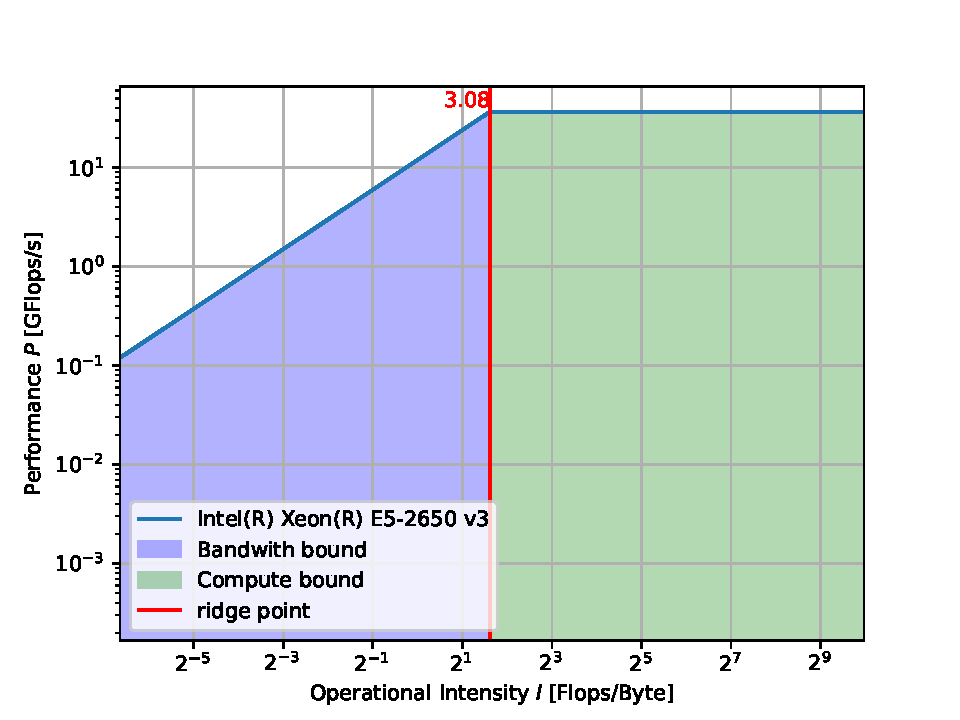
\includegraphics[width=\textwidth]{../media/roofline.pdf}
	\caption{Naive roofline model for Intel Xeon E5-2650 v3 @ 2.30GHz}
	\label{fig:roofline}
\end{figure}




